\documentclass[tikz,border=6pt]{standalone}
\usepackage{stanli}%<--stanli
\tikzset{every node/.style={font=\footnotesize}}

\newcommand{\h}{1.6}
\newcommand{\dicke}{0.6}

\pgfmathsetmacro{\hminus}{\h - \dicke/2}
\pgfmathsetmacro{\hplus}{\h + \dicke/2}

\tikzset{
  pics/FZRS/.style={
    code={
      \draw[thin] (0,0.7) -- (0.3,0.7);
      \draw[thin] (0,1) -- (0.5,1);
      
      \draw[thin] (0,0.725) -- (0.3,0.725);
      \draw[thin] (0,0.975) -- (0.3,0.975);
      
      \draw[thin] (0,1) -- (0,0.7);
      
      \draw[thin] (0.025,0.975) -- (0.025,0.725);
      
      \draw[thin] (0.5,1) -- (0.5,0);
      \draw[thin] (0.3,1) -- (0.3,0);
      
      \draw[thin] (0.475,1) -- (0.475,0);
      \draw[thin] (0.325,1) -- (0.325,0);
    }
  },
  pics/diagonaltotheright/.style={
    code={
      \draw[red, thin] (0,0) -- (2.8,-4);
    }
  },
  pics/diagonaltotheleft/.style={
    code={
      \draw[red, thin] (0,0) -- (-2.8,-4);
    }
  }
}



\begin{document}
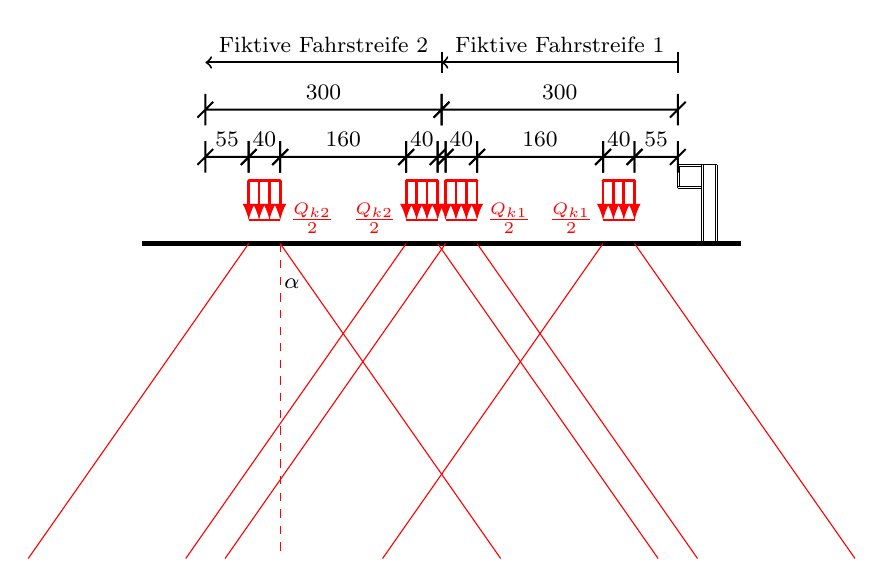
\begin{tikzpicture}
\scaling{1}
\point{SN1}{-0.8}{0}
\point{S0}{0}{0}
\point{S1}{0.55}{0}
\point{S2}{0.95}{0}
\point{alpha}{1.1}{-0.7}
\point{S3}{2.55}{0}
\point{S4}{2.95}{0}
\point{S5}{3}{0}
\point{S6}{3.05}{0}
\point{S7}{3.45}{0}
\point{S8}{5.05}{0}
\point{S9}{5.45}{0}
\point{S10}{6}{0}
\point{S11}{6.8}{0}


%\notation{6}{SN1}{+}
%\notation{6}{S0}{+}
%\notation{6}{S1}{+}
%\notation{6}{S2}{+}
%\notation{6}{S3}{+}
%\notation{6}{S4}{+}
%\notation{6}{S5}{+}
%\notation{6}{S6}{+}
%\notation{6}{S7}{+}
%\notation{6}{S8}{+}
%\notation{6}{S9}{+}
%\notation{6}{S10}{+}
%\notation{6}{S10_1}{+}
%\notation{6}{S10_2}{+}
%\notation{6}{S10_3}{+}
%\notation{6}{S11}{+}




%Strasselinien
\beam{2}{SN1}{S11}


%%Loads
\begin{scope}[color=red]
\lineload{1}{S1}{S2}[0.5][0.5][0.33];
\lineload{1}{S3}{S4}[0.5][0.5][0.33];
\lineload{1}{S6}{S7}[0.5][0.5][0.33];
\lineload{1}{S8}{S9}[0.5][0.5][0.33];
%NameLoads
\notation{1}{S2}{$\frac{Q_{k2}}{2}$}[above right]
\notation{1}{S3}{$\frac{Q_{k2}}{2}$}[above left]
\notation{1}{S7}{$\frac{Q_{k1}}{2}$}[above right]
\notation{1}{S8}{$\frac{Q_{k1}}{2}$}[above left]
\end{scope}
\dimensioning{1}{S0}{S1}{1.1}[55];
\dimensioning{1}{S1}{S2}{1.1}[40];
\dimensioning{1}{S2}{S3}{1.1}[160];
\dimensioning{1}{S3}{S4}{1.1}[40];
\dimensioning{1}{S4}{S6}{1.1};
\dimensioning{1}{S6}{S7}{1.1}[40];
\dimensioning{1}{S7}{S8}{1.1}[160];
\dimensioning{1}{S8}{S9}{1.1}[40];
\dimensioning{1}{S9}{S10}{1.1}[55];

\dimensioning{1}{S0}{S5}{1.7}[300];
\dimensioning{1}{S5}{S10}{1.7}[300];
 % NameDimensions
\dimensioning{3}{S5}{S0}{-2.3}[Fiktive Fahrstreife 2];
\dimensioning{3}{S10}{S5}{-2.3}[Fiktive Fahrstreife 1];


\pic at (S10) {FZRS};
\pic at (S2) {diagonaltotheright};
\draw[red, thin,dashed] (0.95,0) -- (0.95,-4);
\notation{1}{alpha}{$\alpha$}[above]
\pic at (S4) {diagonaltotheright};
\pic at (S7) {diagonaltotheright};
\pic at (S9) {diagonaltotheright};
\pic at (S1) {diagonaltotheleft};
\pic at (S3) {diagonaltotheleft};
\pic at (S6) {diagonaltotheleft};
\pic at (S8) {diagonaltotheleft};





\end{tikzpicture}
\end{document}
